\subsection{Casos de Uso}
\subsubsection{Diagrama de casos de uso}
En esta sección intentaremos terminar de definir de manera más precisa y detallada las diferentes interacciones que puedan existir entre nuestro sistema y los diferentes actores. Para ello utilizaremos el modelado con un diagrama de casos de uso.


\begin{figure}[H]
    \centering
    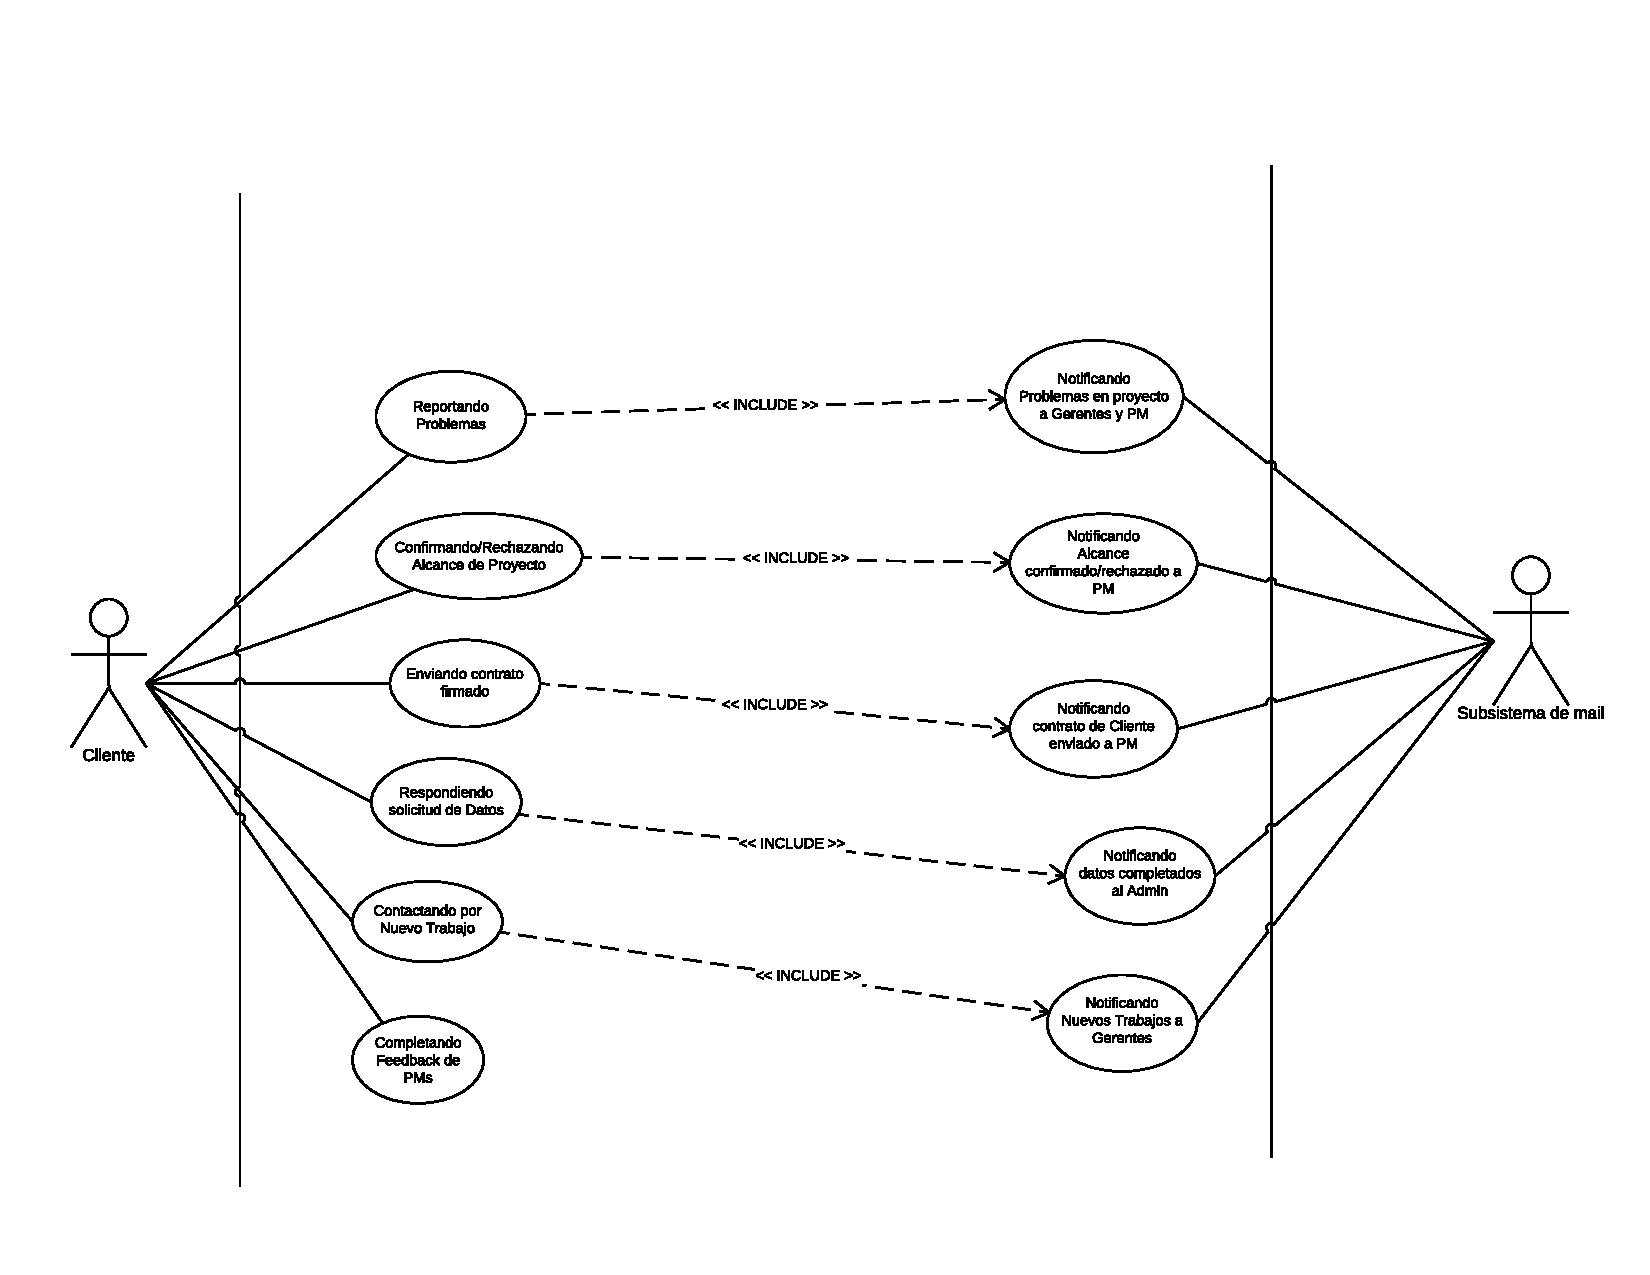
\includegraphics[width=\linewidth]{diag/viejos/cu1.pdf}
    \caption{Casos de Uso: Cliente y Subsistema de Mail}
    \label{cu1}
\end{figure}

\begin{figure}[H]
    \centering
    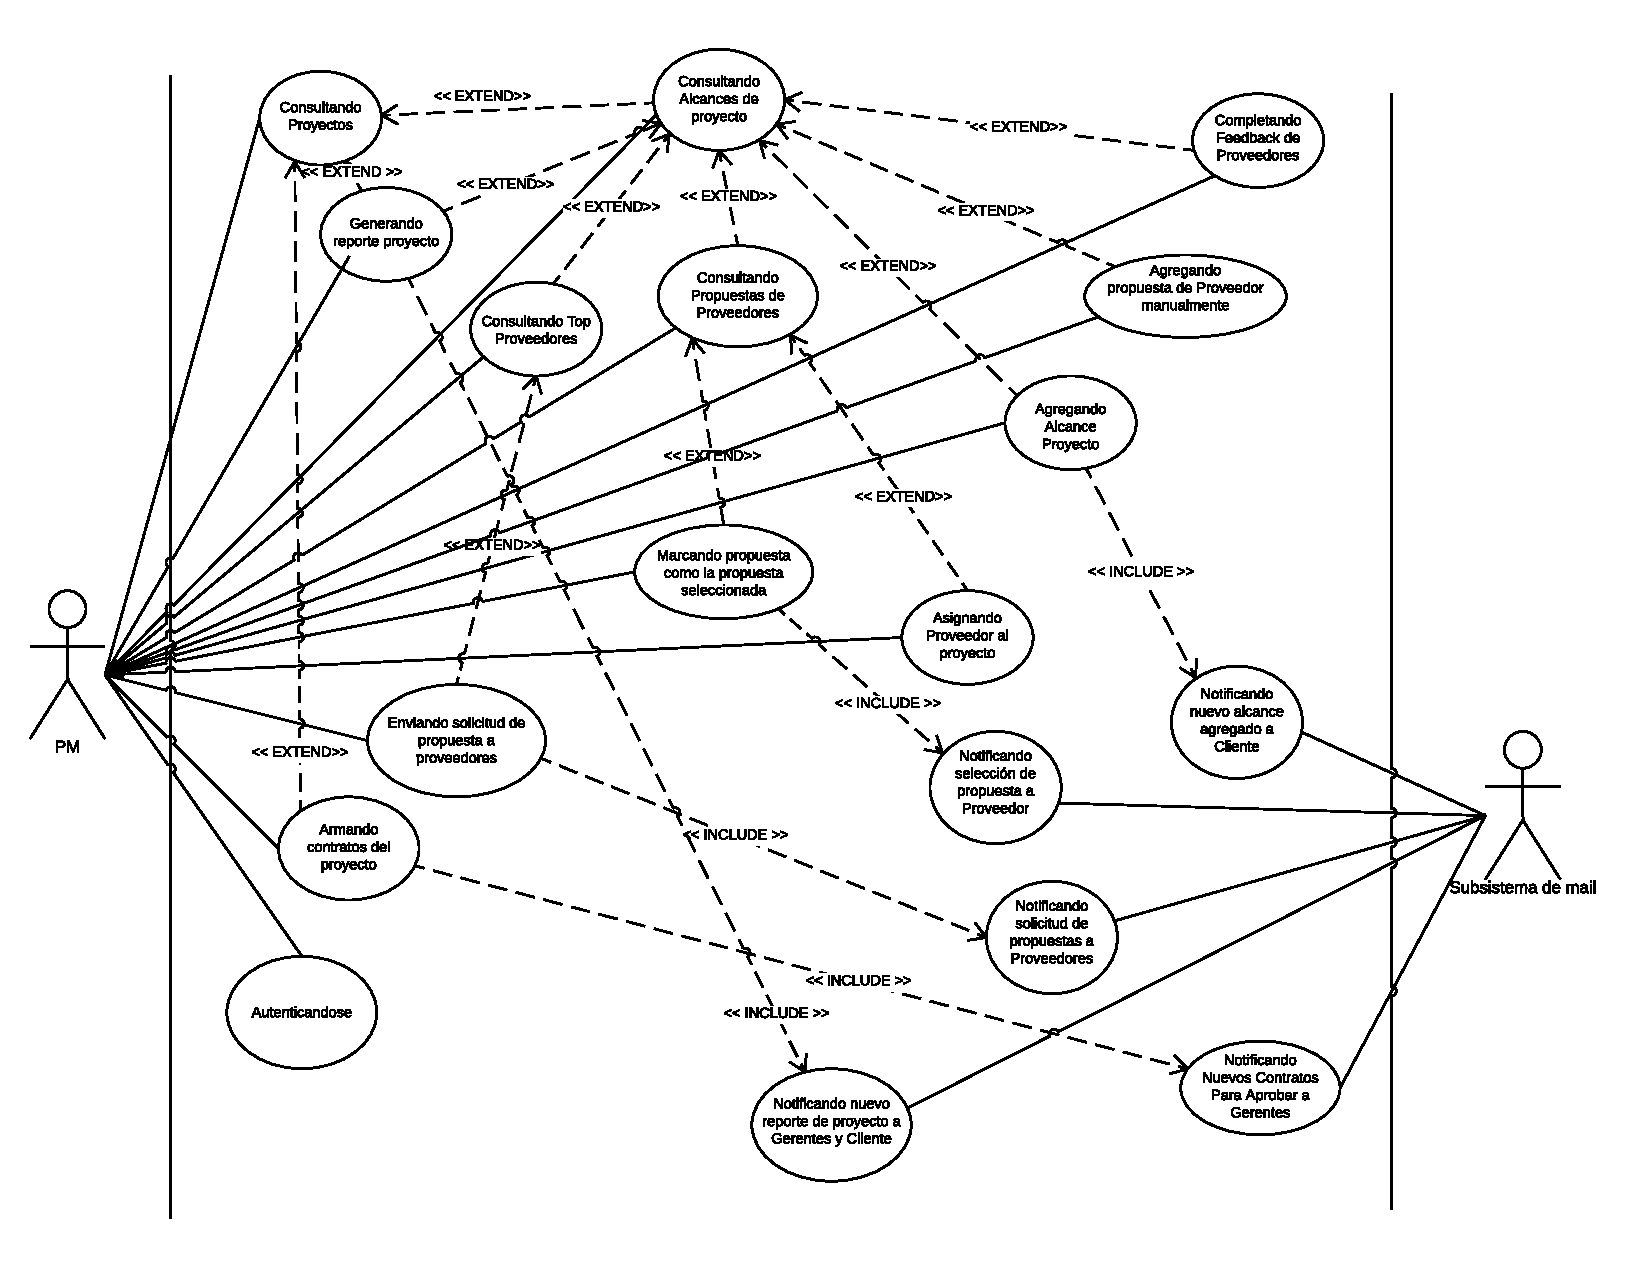
\includegraphics[width=\linewidth]{diag/viejos/cu2.pdf}
    \caption{Casos de Uso: PM y Subsistema de Mail}
    \label{cu2}
\end{figure}

\begin{figure}[H]
    \centering
    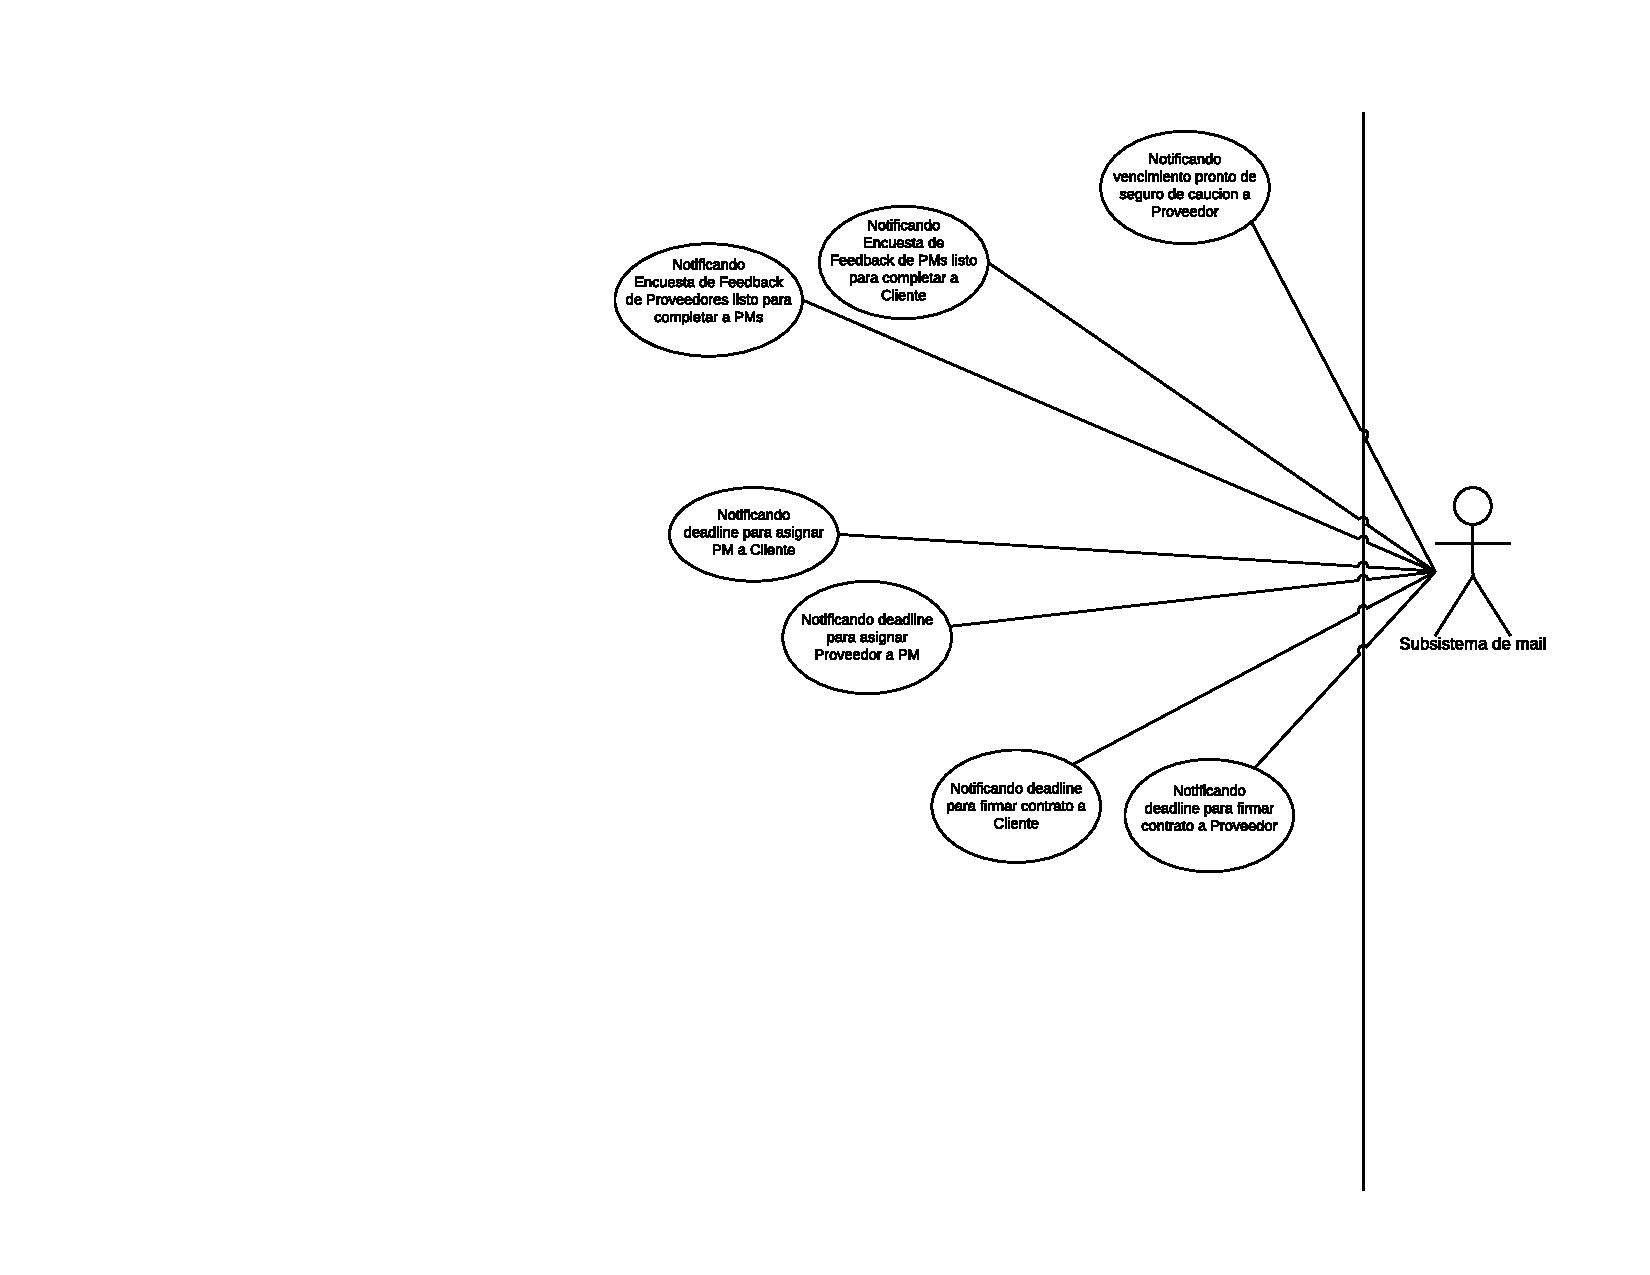
\includegraphics[width=\linewidth]{diag/viejos/cu3.pdf}
    \caption{Casos de Uso: Subsistema de Mail}
    \label{cu3}
\end{figure}

\begin{figure}[H]
    \centering
    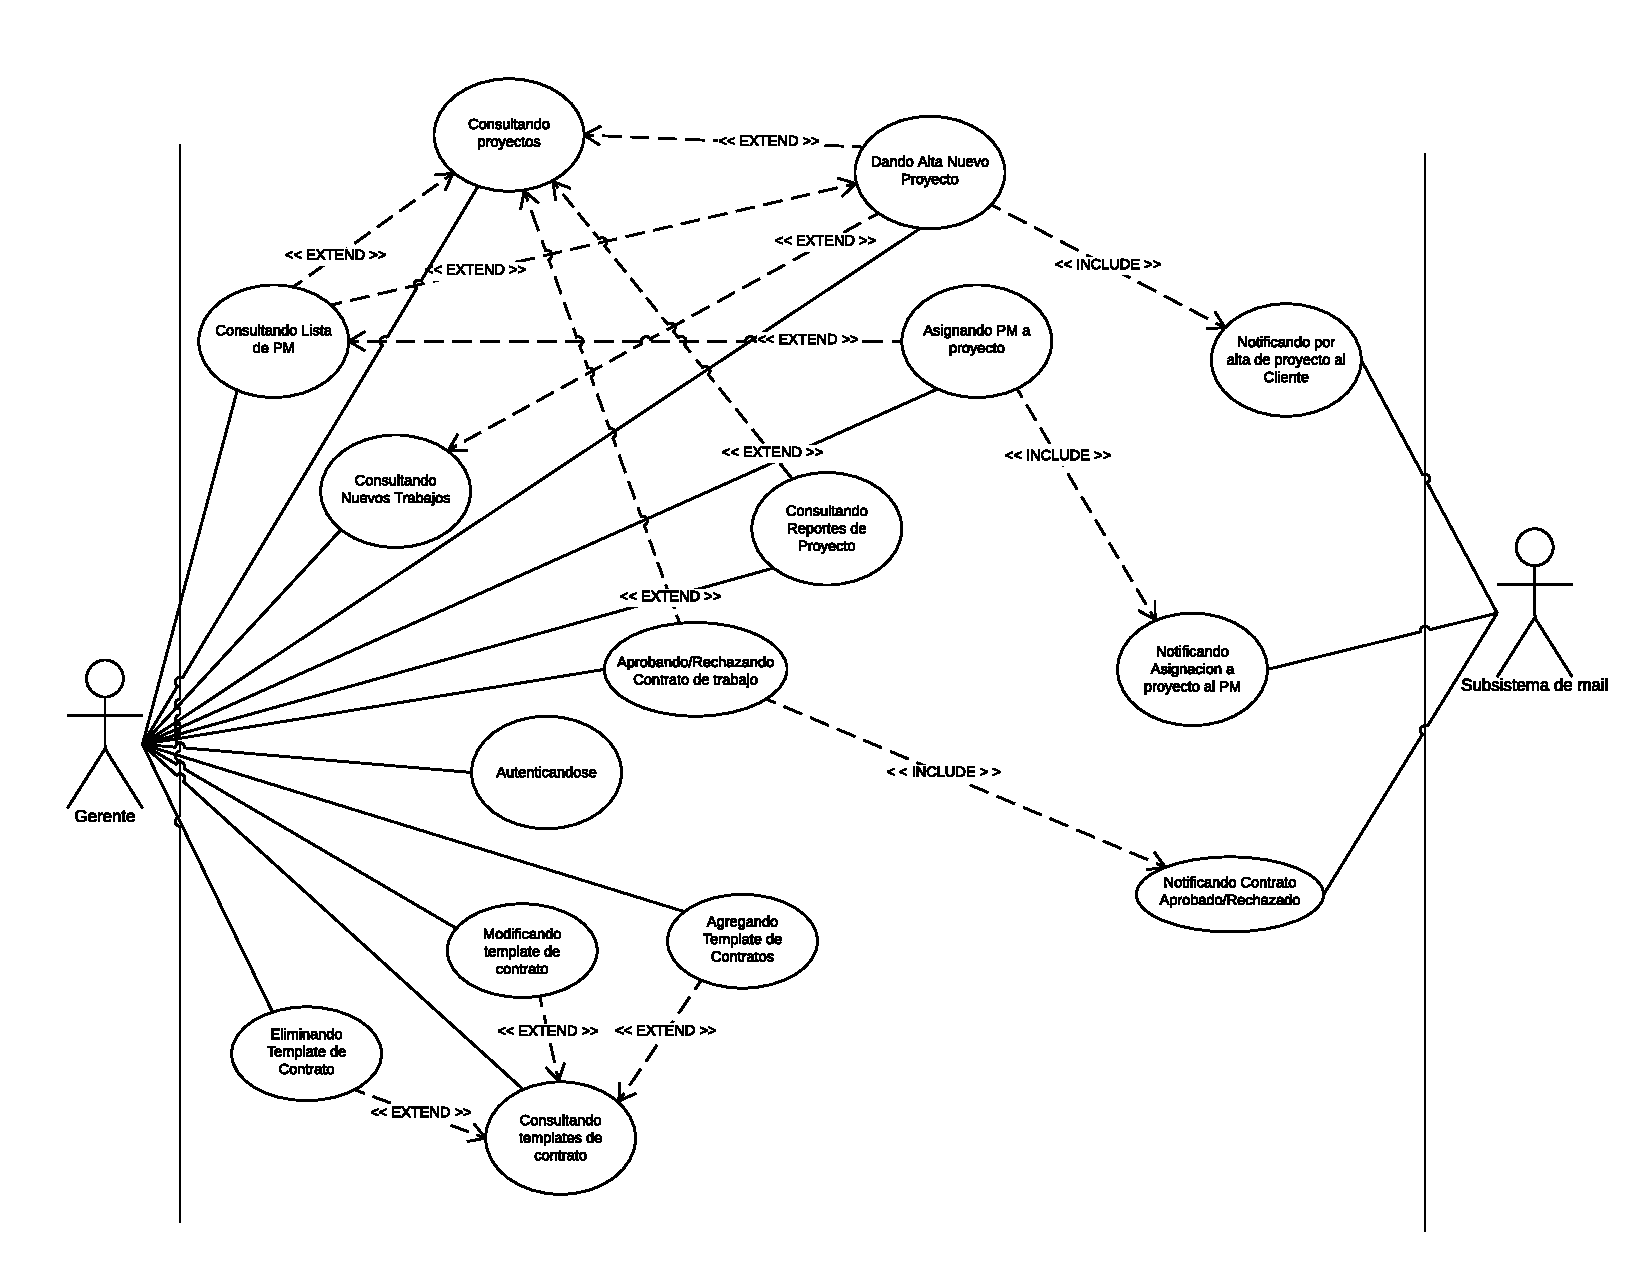
\includegraphics[width=\linewidth]{diag/viejos/cu4.pdf}
    \caption{Casos de Uso: Gerente y Subsistema de Mail}
    \label{cu4}
\end{figure}

\begin{figure}[H]
    \centering
    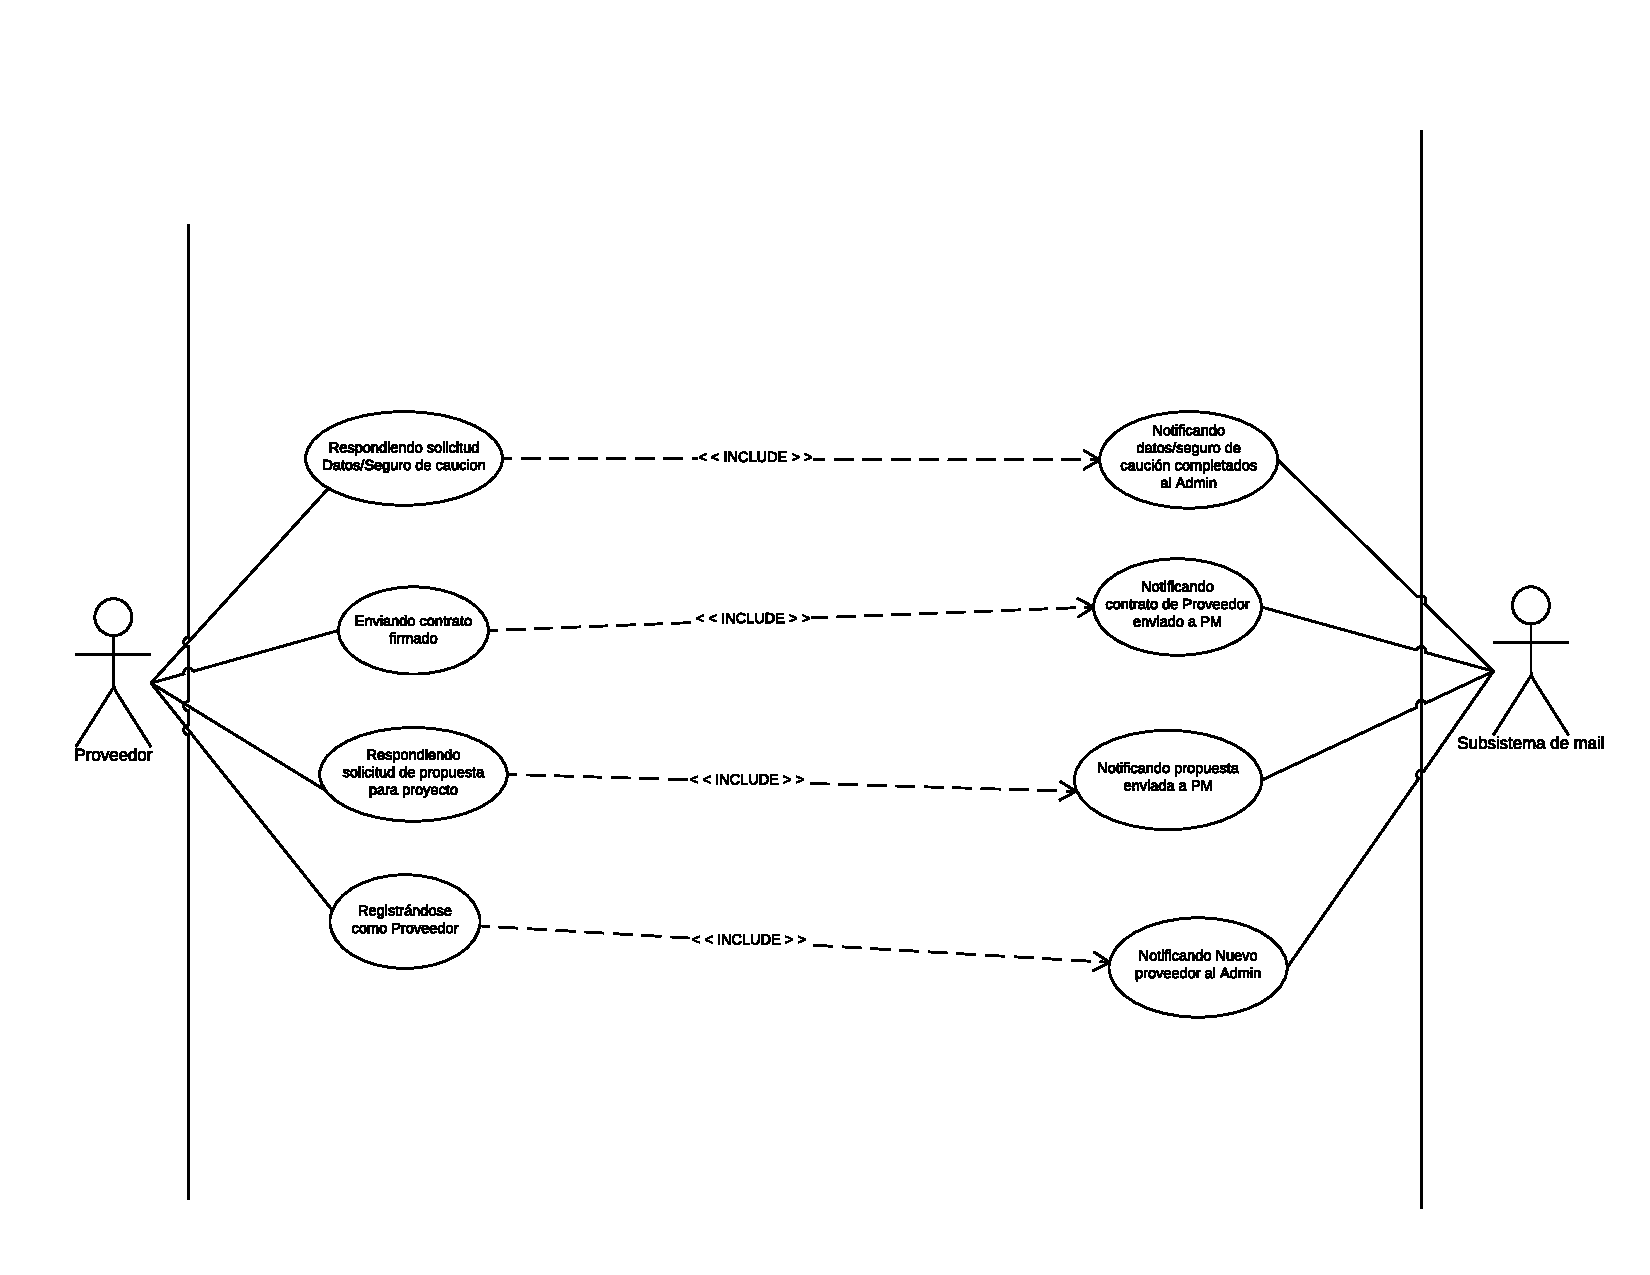
\includegraphics[width=\linewidth]{diag/viejos/cu5.pdf}
    \caption{Casos de Uso: Proveedor y Subsistema de Mail}
    \label{cu5}
\end{figure}

\begin{figure}[H]
    \centering
    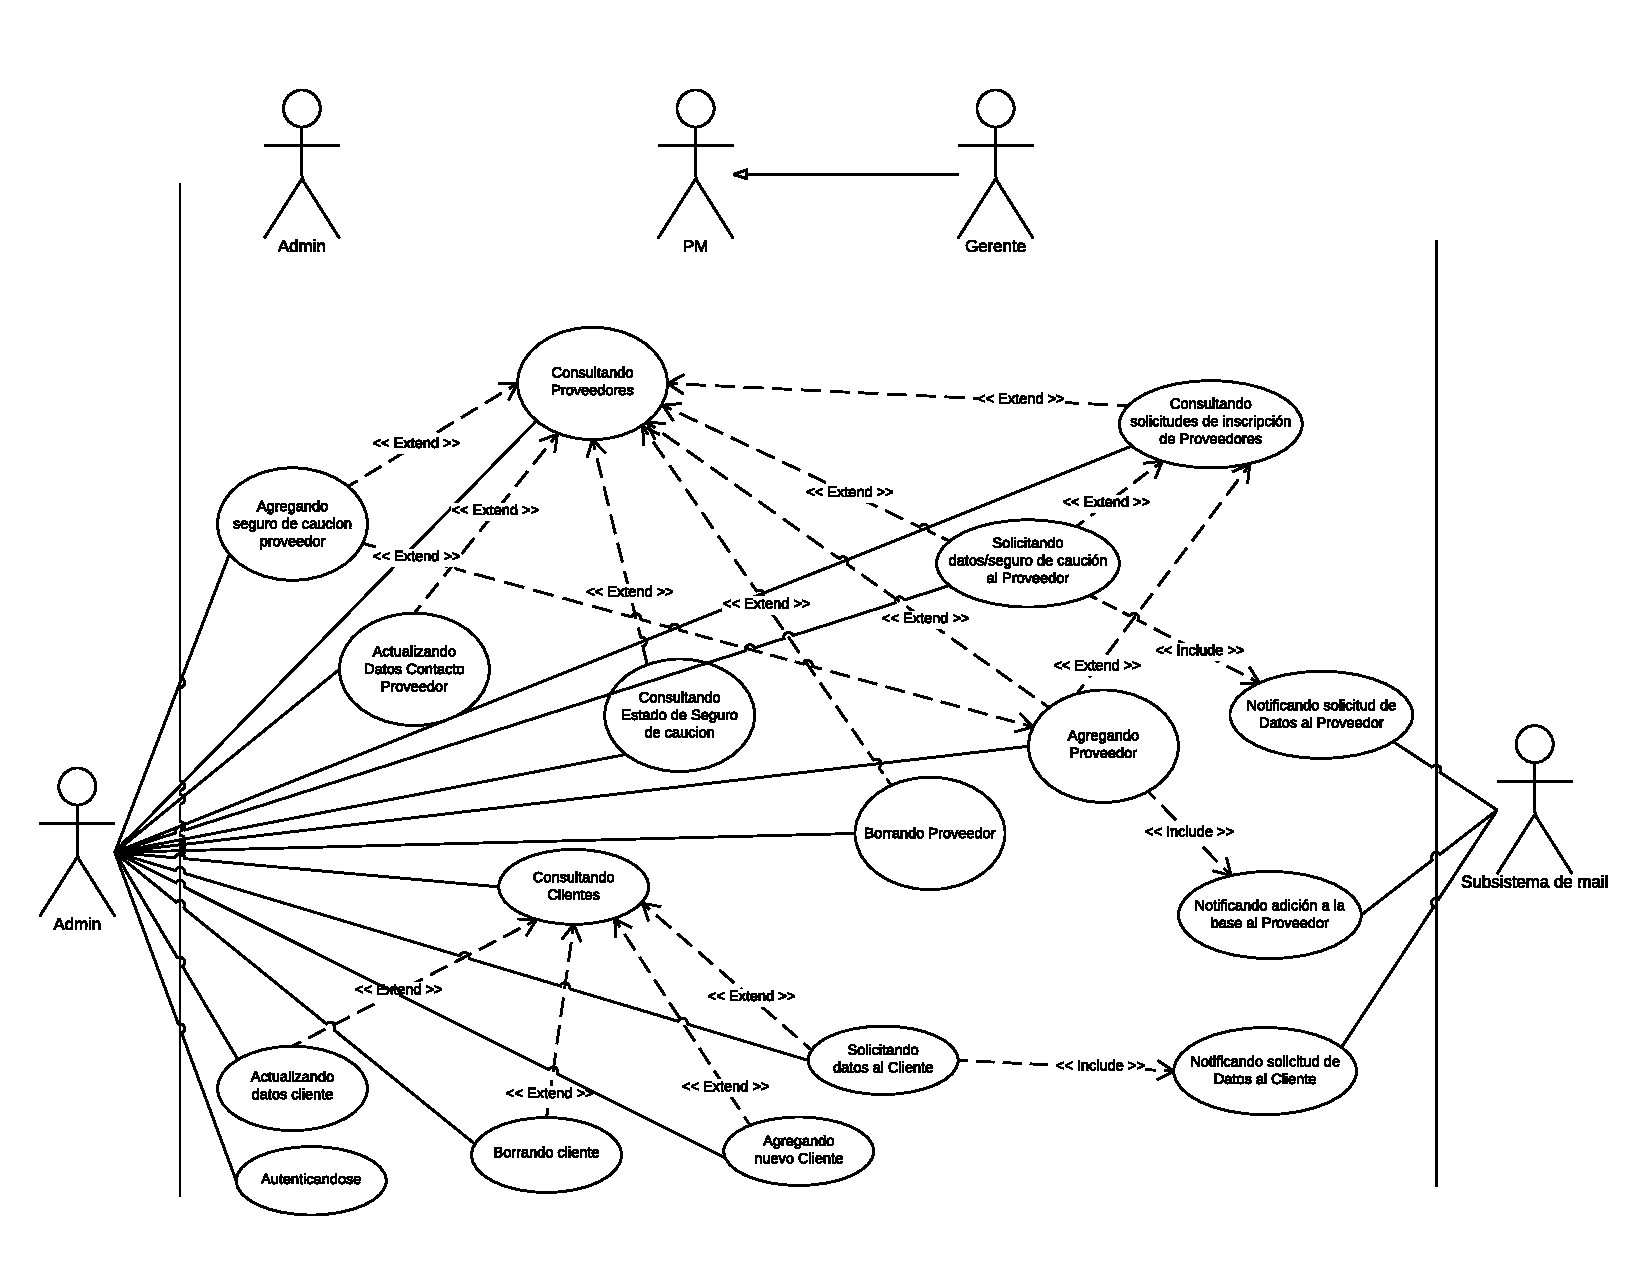
\includegraphics[width=\linewidth]{diag/viejos/cu6.pdf}
    \caption{Casos de Uso: Administrador y Subsistema de Mail}
    \label{cu6}
\end{figure}

\subsubsection{Detalles}
Para finalizar detallaremos los distintos casos de uso en los que además intentaremos ver cuáles son los comportamientos alternativos que pueda tener nuestro sistema en las distintas circunstancias.


% ADMIN
\subsubsection{Detalles de Casos de Uso del Administrador}
\begin{longtable}{| p{.60\textwidth} | p{.40\textwidth} |}
    \hline
    \multicolumn{2}{|p{16cm}|}{
        \textbf{Caso de uso:} Consultando Proveedores \newline
        \textbf{Actor:} Administrador\newline
        \textbf{Pre:}  True\newline
        \textbf{Post:}El Administrador consulta el proveedor.
    }\\
    \hline
    1.El sistema le solicita que ingrese los filtros de búsqueda  & \\
    \hline
    2.El Administrador Agrega los datos del proveedor que está buscando& \\
    \hline
    3.El Sistema encuentra el proveedor y muestra los datos de contacto & 3.1.El proveedor solicitado no se encuentra en el sistema \newline 3.2 Fin de C.U.  \\
    \hline
    4.El Administrador decide eliminar el proveedor. Extiende Caso de uso Borrando Proveedor.& \\
    \hline
    5.El Administrador decide agregar el seguro de Caución de proveedor. Extiende Caso de uso Agregando Seguro de Caución.& \\
    \hline
    6.El Administrador decide consultar estado del seguro de Caución de proveedor. Extiende Caso de uso Consultando estado de seguro de caución.& \\
    \hline
    7.El Administrador decide actualizar datos del proveedor. Extiende Caso de uso Actualizando datos de proveedor.& \\
    \hline
    8.Fin de C.U.& \\
    \hline
\end{longtable}


\begin{longtable}{| p{.60\textwidth} | p{.40\textwidth} |}
    \hline
    \multicolumn{2}{|p{16cm}|}{
        \textbf{Caso de uso:} Consultando Clientes \newline
        \textbf{Actor:} Administrador\newline
        \textbf{Pre:}  True\newline
        \textbf{Post:}El Administrador Consulta los clientes.
    }\\
    \hline
    1.El sistema le solicita que ingrese los filtros de busqueda  & \\
    \hline
    2.El Administrador Agrega los datos del cliente que está buscando& \\
    \hline
    3.El Sistema encuentra el cliente y muestra los datos de contacto & 3.1.El cliente solicitado no se encuentra en el sistema \newline 3.2 Fin de C.U.  \\
    \hline
    4.El Administrador decide eliminar el clientes. Extiende Caso de uso Borrando cliente.& \\
    \hline
    5.El Administrador decide actualizar datos del cliente. Extiende Caso de uso Actualizando datos cliente.& \\
    \hline
    6.El Administrador Agregar un nuevo cliente. Extiende Caso de uso Agregando nuevo Cliente.& \\
    \hline
    7.El Administrador decide Solicitar Datos al cliente. Extiende Caso de uso Solicitando datos al Cliente.& \\
    \hline
    8.Fin de C.U.& \\
    \hline
\end{longtable}

\begin{longtable}{| p{.60\textwidth} | p{.40\textwidth} |}
    \hline
    \multicolumn{2}{|p{16cm}|}{
        \textbf{Caso de uso:} Agregando Proveedor \newline
        \textbf{Actor:} Administrador\newline
        \textbf{Pre:}  True\newline
        \textbf{Post:} El proveedor fue agregado al sistema
    }\\
    \hline
    1.El sistema le solicita que ingrese los datos de contacto del proveedor & \\
    \hline
    2.El Administrador Agrega los datos del proveedor como son nombres, datos de contacto y datos relacionados al negocio` &  \\
    \hline
    3.El Sistema valida los datos de contacto para ver si no se encuentra registrado & 3.1.El proveedor ya está dado de alta \newline 3.2 Fin de C.U.  \\
    \hline
    4.El Sistema Pregunta si desea Agregar el seguro de caución&\\
    \hline
    5.El Administrador Agrega Seguro de caución, Extiende Caso de Uso Agregar seguro de Caucion. & 5.1 El Administrador decide agregarlo luego. Continua en paso 5 \\
    \hline
    6.El Sistema Guarda el proveedor. USA Notificando adición a la base de proveedores& \\
    \hline
    7.Fin de C.U.& \\
    \hline
\end{longtable}

\begin{longtable}{| p{.60\textwidth} | p{.40\textwidth} |}
    \hline
    \multicolumn{2}{|p{16cm}|}{
        \textbf{Caso de uso:} Borrando Proveedor \newline
        \textbf{Actor:} Administrador\newline
        \textbf{Pre:}  Proveedor Seleccionado\newline
        \textbf{Post:} El proveedor fue eliminado del sistema
    }\\
    \hline
    1.El sistema  muetra las opciones para realizar con un proveedor & \\
    \hline
    2.El Administrador selecciona eliminar& \\
    \hline
    3.El Sistema lanza un mensaje consultando si desea eliminar el proveedor &  \\
    \hline
    4.El Administrador selecciona que SI desea eliminar el proveedor & 4.1.1 El Sistema nota que el proveedor sigue asignado a un proyecto en curso, muestra un mensaje por pantalla notificando este problema \newline 4.1.2 Fin Caso de Uso \newline 4.2.1 El usuario Selecciona que NO desea eliminar el proveedor \newline4.2.2 Fin de Caso de uso\\
    \hline
    5.El Sistema elimina el proveedor del sistema &  \\
    \hline
    6.Fin de C.U.& \\
    \hline
\end{longtable}
\begin{longtable}{|p{.60\textwidth}|p{.40\textwidth}|}
    \hline
    \multicolumn{2}{|p{16cm}|}{
        \textbf{Caso de uso:} Actualizando datos de contacto de Proveedor \newline
        \textbf{Actor:} Administrador\newline
        \textbf{Pre:}  Proveedor seleccionado\newline
        \textbf{Post:} El Administrador actualiza los datos del Proveedor
    }\\
    \hline
    1.El sistema  muestra las opciones para realizar con un proveedor & \\
    \hline
    2.El Administrador selecciona Actualizar Datos Proveedor&   \\
    \hline
    3.El Sistema muestra todos los campos con los datos del proveedor para modificar y dos botones , uno para guardar y otro para cancelar&  \\
    \hline
    4.El Administrador Modifica los datos y toca salvar & 4.1.El Administrador toca cancelar \newline 4.2 Fin Caso de Uso \\
    \hline
    5.El Sistema guarda los cambios al proveedor &  \\
    \hline
    6.Fin de C.U.& \\
    \hline
\end{longtable}

\begin{longtable}{|p{.60\textwidth}|p{.40\textwidth}|}
    \hline
    \multicolumn{2}{|p{16cm}|}{
        \textbf{Caso de uso:} Consultando estado de seguro de caución \newline
        \textbf{Actor:} Administrador\newline
        \textbf{Pre: }  Proveedor seleccionado \newline
        \textbf{Post:} El Administrador consulta estado del seguro de caución
    }\\
    \hline
    1.El Administrador selecciona la opción consultar estado de seguro de caución&  \\
    \hline
    2.El Sistema muestra el estado de seguro de caucion&  \\
    \hline
    3.Fin de C.U.& \\
    \hline
\end{longtable}

\begin{longtable}{|p{.60\textwidth}|p{.40\textwidth}|}
    \hline
    \multicolumn{2}{|p{16cm}|}{
        \textbf{Caso de uso:} Agregando seguro de caucion\newline
        \textbf{Actor:} Administrador\newline
        \textbf{Pre: }  Proveedor seleccionado\newline
        \textbf{Post:} El Administrador Agrega un nuevo seguro de caución
    }\\
    \hline
    1.El Administrador selecciona la opción agregar de seguro de caucion& \\
    \hline
    2.El Sistema muestra la opción de ingreso de validez del seguro de caución y el ingreso del archivo con el seguro de caucion&  \\
    \hline
    3.El Administrador ingresa la fecha de validez, agrega el archivo del escaneo del seguro de caucion y guarda los cambios&3.1 El administrador aprieta el botón cancelar \newline 3.2 Fin del Caso de uso \\
    \hline
    4.El Sistema verifica la fecha de validez y que no que no exista otro seguro de caución & \\
    \hline
    5.El Sistema aprueba los datos ingresados y guarda los cambios &5.1.1 Los datos ingresados son incorrectos, el sistema muestra mensaje de error \newline 5.1.2 vuelve al paso 4 \newline 5.2.1 Existe otro seguro de caución en la misma fecha, el sistema muestra un mensaje avisando que actualizara los datos con el nuevo seguro de caución. \newline 5.2 vuelve al paso 4\\
    \hline
    6.Fin de C.U.& \\
    \hline
\end{longtable}

\begin{longtable}{|p{.60\textwidth}|p{.40\textwidth}|}
    \hline
    \multicolumn{2}{|p{16cm}|}{
        \textbf{Caso de uso:} Solicitando datos/seguro de caucion de proveedor\newline
        \textbf{Actor:} Administrador\newline
        \textbf{Pre:} Proveedor seleccionado\newline
        \textbf{Post:} El Administrador Agrega un nuevo seguro de caucion
    }\\
    \hline
    1.El sistema  muestra las opciones para realizar con un proveedor & \\
    \hline
    2.El Administrador selecciona la opción agregar de seguro de caucion& \\
    \hline
    3.El Sistema muestra la opcion de ingreso de validez del seguro de caucion y el ingreso del archivo con el seguro de caucion&  \\
    \hline
    4.El Administrador ingresa la fecha de validez, agrega el archivo del escaneo del seguro de caucion y guarda los cambios&4.1 El administrador Apreta el boton cancelar \newline 4.2 Fin del Caso de uso \\
    \hline
    5.El Sistema verifica la fecha de validez y que no que no exista otro seguro de caucion & \\
    \hline
    6.El Sistema aprueba los datos ingresados y guarda los cambios &6.1 Los datos ingresados son incorrectos, o hay otro seguro de caucion en la misma fecha  \newline 6.2 vuelve al paso 4\\
    \hline
    7.Fin de C.U.& \\
    \hline
\end{longtable}


% cliente
\subsubsection{Detalles de Casos de Uso del Cliente}
\begin{longtable}{|p{.60\textwidth}|p{.40\textwidth}|}
    \hline
    \multicolumn{2}{|p{16cm}|}{
        \textbf{Caso de uso:} Contactando por nuevos trabajos\newline
        \textbf{Actor:} Cliente\newline
        \textbf{Pre: }  True\newline
        \textbf{Post:} El Cliente deja el contacto para un nuevo trabajo en el sistema
    }\\
    \hline
    1.El Cliente selecciona la opción de contacto por nuevos trabajos y completa los datos de contacto&2.1 El Cliente no ingresa datos de contacto\newline 1.2 Fin caso de uso   \\
    \hline
    2.El Sistema notifica nuevo proyecto. USA Notificando nuevos trabajos a gerente& \\
    \hline
    3.Fin de C.U.& \\
    \hline
\end{longtable}


\begin{longtable}{|p{.60\textwidth}|p{.40\textwidth}|}
    \hline
    \multicolumn{2}{|p{16cm}|}{
        \textbf{Caso de uso:} Completando Feedback de PM\newline
        \textbf{Actor:} Cliente\newline
        \textbf{Pre: }El Cliente Accede al sistema con link Provisto en alta de proyecto\newline
        \textbf{Post: }El Cliente Completo la encuesta
    }\\
    \hline
    1.El Usuario accede al link que recibió en el Mail y le abre una página web con la encuesta a completar & 1.1.El Usuario desestima el mail .\newline 1.2Fin de C.U.\\
    \hline
    2.El Sistema Muestra un formulario con un área de texto libre para completar sobre el feedback del PM &\\
    \hline
    3.El Usuario Completa el formulario y Apreta la opción de enviar el formulario& \\
    \hline
    4.El Sistema Registra la nueva encuesta&\\
    \hline
    5.El Sistema actualiza el puntaje del PM&\\
    \hline
    6.Fin del C.U&\\
    \hline
\end{longtable}

\begin{longtable}{|p{.60\textwidth}|p{.40\textwidth}|}
    \hline
    \multicolumn{2}{|p{16cm}|}{
        \textbf{Caso de uso:} Reportando Problemas\newline
        \textbf{Actor:} Cliente\newline
        \textbf{Pre: }El Cliente Accede al sistema con link Provisto en alta de proyecto\newline
        \textbf{Post: }El Cliente notifico de un problema
    }\\
    \hline
    1.El Usuario entra a la página web con el link provisto y selecciona la opción reportar problema.&\\
    \hline
    2.El Sistema muestra un formulario con espacio para escribir un detalle del problema&    \\
    \hline
    3.El Cliente Completa dicho formulario y selecciona la opción Enviar& \\
    \hline
    4.El Sistema Registra el problema. Extiende Notificando Problemas en Proyectos a gerentes y PM&\\
    \hline
    5.Fin del C.U&\\
    \hline
\end{longtable}

\begin{longtable}{|p{.60\textwidth}|p{.40\textwidth}|}
    \hline
    \multicolumn{2}{|p{16cm}|}{
        \textbf{Caso de uso:} Enviando Contrato firmado \newline
        \textbf{Actor:} Cliente\newline
        \textbf{Pre: }El Cliente Accede al sistema con link Provisto en alta de proyecto\newline
        \textbf{Post: }El Envio el contrato firmado
    }\\
    \hline
    1.El Usuario entra a la página web con el link provisto y selecciona la opción enviar contrato.&\\
    \hline
    2.El Sistema pide que selección el archivo pdf firmado desde su computadora&    \\
    \hline
    3.El Cliente Selecciona el archivo.& \\
    \hline
    4.El Sistema Guarda el contrato firmado. Extiende Notificando contrato de Cliente enviado a PM&\\
    \hline
    5.Fin del C.U&\\
    \hline
\end{longtable}

\begin{longtable}{|p{.60\textwidth}|p{.40\textwidth}|}
    \hline
    \multicolumn{2}{|p{16cm}|}{
        \textbf{Caso de uso:} Respondiendo solicitud de Datos \newline
        \textbf{Actor:} Cliente\newline
        \textbf{Pre: }El Cliente Accede al sistema con link Provisto en mail de solicitud\newline
        \textbf{Post: }El cliente completa datos pendientes
    }\\
    \hline
    1.El Usuario entra a la página web con el link provisto.&\\
    \hline
    2.El Sistema Presenta un formulario con datos obligatorios como teléfono, ubicación, nombre, datos del negocio, servicios y productos que ofrece &    \\
    \hline
    3.El Cliente Completa los datos y presiona el botón guardar. &3.1 El Cliente no completa los datos.\newline 3.2 El Sistema lo marca como incompleto.\newline 3.3 Fin del C.U.\\
    \hline
    4.El Sistema Guarda los datos. Extiende Notificando datos completados al Admin&\\
    \hline
    5.Fin del C.U&\\
    \hline
\end{longtable}


% PM
\subsubsection{Detalles de Casos de Uso del PM}
\begin{longtable}{|p{.60\textwidth}|p{.40\textwidth}|}
    \hline
    \multicolumn{2}{|p{16cm}|}{
        \textbf{Caso de uso:}Consultando Proyectos\newline
        \textbf{Actor:} PM\newline
        \textbf{Pre: }El PM esta autenticado en el sistema\newline
        \textbf{Post:} El PM ve todos los proyectos registrados en el sistema
    }\\
    \hline
    1.El PM selecciona buscar proyectos& \\
    \hline
    2.El sistema muestra todos los proyectos disponibles en forma de lista mostrando nombre del cliente y nombre del proyecto &\\
    \hline
    3.El PM decide filtrar por Cliente y selección la opción de filtrar por cliente& \\
    \hline
    4.El PM escribe el nombre del Cliente& \\
    \hline
    5.El Sistema lista todos los resultados de búsqueda&\\
    \hline
    6.Fin del C.U.&\\
    \hline
\end{longtable}

\begin{longtable}{|p{.60\textwidth}|p{.40\textwidth}|}
    \hline
    \multicolumn{2}{|p{16cm}|}{
        \textbf{Caso de uso:}Consultando alcance de Proyectos\newline
        \textbf{Actor:} PM\newline
        \textbf{Pre: }Proyecto Seleccionado\newline
        \textbf{Post:} El PM Puede ve los alcances de un proyecto
    }\\
    \hline
    1.El Pm Busca un proyecto. Extiende Consultando Proyectos& \\
    \hline
    2.El PM selecciona ver los alcances del proyecto&  \\
    \hline
    3.El sistema muestra los alcances del proyectos& \\
    \hline
    4.Fin del C.U&\\
    \hline
\end{longtable}

\begin{longtable}{|p{.60\textwidth}|p{.40\textwidth}|}
    \hline
    \multicolumn{2}{|p{16cm}|}{
        \textbf{Caso de uso:}Consultando TOP de proveedores\newline
        \textbf{Actor:} PM\newline
        \textbf{Pre: }Proyecto Seleccionado\newline
        \textbf{Post:} El PM obtiene una lista de proveedores ordenados según los filtros seleccionados
    }\\
    \hline
    1.El sistema muestra los filtros de búsqueda como nombre de proveedor, datos del negocio o ubicación. & \\
    \hline
    2.El PM completa los filtros de búsqueda que necesita&  \\
    \hline
    3.El sistema muestra los resultados basado en los filtros de búsqueda ordenados por algun criterio seleccionado& \\
    \hline
    4.El PM Selecciona Proveedor &\\
    \hline
    5.El PM Desea enviar una solicitud de presupuesto. Extiende Solicitud de propuesta a proveedores &5.1 El PM Desea seguir viendo otros proveedores y presiona el botón retroceder \newline 5.2 Continua en el paso 3\\
    \hline
    6.Fin del C.U&\\
    \hline
\end{longtable}


\begin{longtable}{|p{.60\textwidth}|p{.40\textwidth}|}
    \hline
    \multicolumn{2}{|p{16cm}|}{
        \textbf{Caso de uso:}Consultando propuestas de los proveedores\newline
        \textbf{Actor:} PM\newline
        \textbf{Pre: }Proyecto Seleccionado\newline
        \textbf{Post:} El PM obtiene una lista de las propuestas presentadas por los proveedores
    }\\
    \hline
    1.El PM selecciona la opción de ver propuestas presentadas&\\
    \hline
    2.El sistema muestra las propuestas presentadas por los distintos proveedores & \\
    \hline
    3.El PM selecciona una propuesta  &\\
    \hline
    4.El sistema muestra el detalle de la propuesta seleccionada sobre productos y costos.&4.1 El PM Desea imprimir la propuesta y selecciona boton Imprimir. \newline 4.2. El PM desea volver a la lista de propuestas. Continua en paso 2\\
    \hline
    5.El PM Desea Asignar el proveedor al proyecto. Extiende Asignando proveedor al proyecto.&\\
    \hline
    6.&\\
    \hline
    5.Fin del C.U&\\
    \hline
\end{longtable}

\begin{longtable}{|p{.60\textwidth}|p{.40\textwidth}|}
    \hline
    \multicolumn{2}{|p{16cm}|}{
        \textbf{Caso de uso:}Marcando una propuesta como seleccionada\newline
        \textbf{Actor:} PM\newline
        \textbf{Pre: }Proyecto Seleccionado\newline
        \textbf{Post:} El PM selecciona una de las propeustas para el proyecto seleccionado
    }\\
    \hline
    1.El PM selecciona una propuesta para el proyecto y guarda los cambios&\\
    \hline
    2.El sistema envía una notificación al proveedor. USA Notificando selección de propuesta a proveedor& 2.1 El Proveedor no notifica como recibida la notificación \newline 2.2 el Sistema no marca como seleccionada la propuesta\\
    \hline
    3.Fin del C.U&\\
    \hline
\end{longtable}

\begin{longtable}{|p{.60\textwidth}|p{.40\textwidth}|}
    \hline
    \multicolumn{2}{|p{16cm}|}{
        \textbf{Caso de uso:}Generando reporte de proyecto\newline
        \textbf{Actor:} PM\newline
        \textbf{Pre: }Proyecto Seleccionado\newline
        \textbf{Post:} El PM agrega un detalle de los avances en el proyecto
    }\\
    \hline
    1.El PM selecciona la opción de agregar reporte &\\
    \hline
    2.El sistema muestra las un formulario para completar con detalles de tareas y fecha, además puede asignar un de estado como crítico, con complicaciones o estable& \\
    \hline
    3.El PM completa un formulario con los avances del proyecto y guarda el reporte&\\
    \hline
    4.El sistema guarda el formulario&\\
    \hline
    5.Fin del C.U&\\
    \hline
\end{longtable}


\begin{longtable}{|p{.60\textwidth}|p{.40\textwidth}|}
    \hline
    \multicolumn{2}{|p{16cm}|}{
        \textbf{Caso de uso:}Enviando solicitud de propuesta a proveedores\newline
        \textbf{Actor:} PM\newline
        \textbf{Pre: }Proyecto Seleccionado\newline
        \textbf{Post:} El PM envía la solicitud de propuestas a los mejores proveedores
    }\\
    \hline
    1.El sistema muestra la lista de TOP de proveedores & \\
    \hline
    2.El PM selecciona varios proveedores y selecciona la opción de enviar solicitud de propuesta& \\
    \hline
    3.El sistema envía la notificación. USA Notificando solicitud de propuestas a proveedores& \\
    \hline
    4.Fin del C.U&\\
    \hline
\end{longtable}

\begin{longtable}{|p{.60\textwidth}|p{.40\textwidth}|}
    \hline
    \multicolumn{2}{|p{16cm}|}{
        \textbf{Caso de uso:}Armando Contrato del Proyecto \newline
        \textbf{Actor:} PM\newline
        \textbf{Pre: }Proyecto Seleccionado\newline
        \textbf{Post:} Arma y agrega contratos al proyecto
    }\\
    \hline
    1.El PM Selecciona Armar Contrato para el proyecto. Extiende Consultando Proyectos & \\
    \hline
    2.El Sistema muestra los templates de contratos de proyectos en el sistema& \\
    \hline
    3.El PM Selecciona un template de contrato& 3.1 El Cliente Desea elegir otro Template y selecciona el botón retornar a lista de contratos. \newline 3.2. Continua en paso 2 \\
    \hline
    4.El PM Completa el Template con los datos del proyecto como datos de Cliente, Proveedores y costos. Presiona Guardar Contrato en proyecto&\\
    \hline
    5.El Sistema Ofrece la opción de imprimir contrato y guarda el contrato como parte del proyecto. USA Notificando Nuevos Contratos Para Aprobar a Gerentes&\\
    \hline
    6.El PM Apreta Aceptar e imprime el contrato.&\\
    \hline
    7.Fin del C.U. &\\
    \hline
\end{longtable}


\begin{longtable}{|p{.60\textwidth}|p{.40\textwidth}|}
    \hline
    \multicolumn{2}{|p{16cm}|}{
        \textbf{Caso de uso:}Cerrando Proyecto \newline
        \textbf{Actor:} PM\newline
        \textbf{Pre: }Proyecto Seleccionado\newline
        \textbf{Post:} Arma y agrega contartos al proyecto
    }\\
    \hline
    1.El PM Selecciona la opción cerrar proyecto. Extiende Consultando Proyectos & \\
    \hline
    2.El Sistema Muestra un mensaje de confirmación& \\
    \hline
    3. El PM Selecciona aceptar & 3.1 El PM Selecciona Cancelar \newline 3.2 Continua en paso 1\\
    \hline
    4.El Sistema marca el proyecto como cerrado. Extiende Notificando Cierre de proyecto y terminacion de obra a gerente &\\
    \hline
    5.Fin de C.U. &\\
    \hline
\end{longtable}

\begin{longtable}{|p{.60\textwidth}|p{.40\textwidth}|}
    \hline
    \multicolumn{2}{|p{16cm}|}{
        \textbf{Caso de uso:}Agregando Propuesta Proveedor Manualmente \newline
        \textbf{Actor:} PM\newline
        \textbf{Pre: }Proyecto Seleccionado\newline
        \textbf{Post:} Agrega una propuesta de proveedor a un proyecto
    }\\
    \hline
    1.El PM Selecciona la opción Agregar Propuesta.& \\
    \hline
    2.El sistema abre una ventana de dialogo donde le solicita el archivo& \\
    \hline
    3. El PM Agrega al archivo y selecciona la opcion guardar & 3.1 El PM Selecciona Cancelar \newline 3.2 Continua en paso 1\\
    \hline
    4.El Sistema Agrega la nueva propuesta&\\
    \hline
    5.Fin de C.U. &\\
    \hline
\end{longtable}

% GERENTE
\subsubsection{Detalles de Casos de Uso del Gerente}
\begin{longtable}{|p{.60\textwidth}|p{.40\textwidth}|}
    \hline
    \multicolumn{2}{|p{16cm}|}{
        \textbf{Caso de uso:}Asignando PM Al Proyecto\newline
        \textbf{Actor:} Gerente\newline
        \textbf{Pre: }Gerente Autenticado\newline
        \textbf{Post:} Un PM es asignado al proyecto
    }\\
    \hline
    1.El Gerente Consulta los proyectos nuevos en el sistema USA Consultando Nuevos Trabajos&    \\
    \hline
    2.El Gerente Consulta los mejores PM para el proyecto dado USA Consultando TOP Proveedores& \\
    \hline
    3.El Gerente Asigna el mejor PM Al Proyecto&\\
    \hline
    4.Fin del C.U&\\
    \hline
\end{longtable}


\begin{longtable}{|p{.60\textwidth}|p{.40\textwidth}|}
    \hline
    \multicolumn{2}{|p{16cm}|}{
        \textbf{Caso de uso:}Consultando Reportes de proyecto\newline
        \textbf{Actor:} Gerente\newline
        \textbf{Pre: }true\newline
        \textbf{Post:}  El Gerente Consulta el estado de un proyecto
    }\\
    \hline
    1.El Gerente Busca un proyecto según ciertos filtros. Extiende Consultando Proyectos&    \\
    \hline
    2.El Sistema le devuelve una lista de proyectos& \\
    \hline
    3.El Gerente Selecciona un proyecto y presiona el botón de obtener estado de proyecto&\\
    \hline
    4.El Sistema Devuelve el estado del proyecto seleccionado &\\
    \hline
    5.Fin del C.U.&\\
    \hline
\end{longtable}

\begin{longtable}{|p{.60\textwidth}|p{.40\textwidth}|}
    \hline
    \multicolumn{2}{|p{16cm}|}{
        \textbf{Caso de uso:}Consultando Nuevos Trabajos\newline
        \textbf{Actor:} Gerente\newline
        \textbf{Pre: }true\newline
        \textbf{Post:}  El Gerente Consulta Nuevos Trabajos
    }\\
    \hline
    1.El Selecciona la opción ver nuevos trabajos&    \\
    \hline
    2.El Sistema le devuelve una lista de nuevos trabajos& \\
    \hline
    3.El Gerente Selecciona un trabajo y desea dar de alta un nuevo proyecto. Extiende Caso de uso Dando Alta Nuevo Proyecto\\
    \hline
    4.Fin del C.U.&\\
    \hline
\end{longtable}

\begin{longtable}{|p{.60\textwidth}|p{.40\textwidth}|}
    \hline
    \multicolumn{2}{|p{16cm}|}{
        \textbf{Caso de uso:}Consultando Nuevos Trabajos\newline
        \textbf{Actor:} Gerente\newline
        \textbf{Pre: }El Gerente consulto nuevos trabajos\newline
        \textbf{Post:}  El Gerente Consulta Nuevos Trabajos
    }\\
    \hline
    1.El Gerente Selecciona  la opción dar de alta nuevos trabajos&    \\
    \hline
    2.El Sistema le consulta si desea agregar un PM al nuevo proyecto& \\
    \hline
    3.El Gerente selecciona la opción SI. Extiende Caso de uso Consultando Lista de PM\\
    \hline
    4.El gerente Guarda los cambios. Usa Caso de uso Notificando Alta de Proyecto&\\
    \hline
    5.Fin C.U&\\
    \hline
\end{longtable}

\begin{longtable}{|p{.60\textwidth}|p{.40\textwidth}|}
    \hline
    \multicolumn{2}{|p{16cm}|}{
        \textbf{Caso de uso:}Consultando Nuevos Trabajos\newline
        \textbf{Actor:} Gerente\newline
        \textbf{Pre: }El Gerente fue notificado de un nuevo Contrato para Aprobar\newline
        \textbf{Post:}  El Gerente Aprueba un contrato de trabajo
    }\\
    \hline
    1.El Gerente Ingresa al Link en el mail donde fue notificado de un nuevo contrato a aprobar&    \\
    \hline
    2.El Sistema le muestra el contrato, y tiene la opción de Aprobar y Rechazar& \\
    \hline
    3.El Gerente selecciona la opción Aprobar. USA Caso de uso Notificando Contrato Aprobado/Rechazado& 3.1 El gerente Selecciona la opción Rechazar. Usa Caso de uso Notificando Contrato Aprobado/Rechazado\\
    \hline
    4.Fin C.U&\\
    \hline
\end{longtable}
\begin{longtable}{|p{.60\textwidth}|p{.40\textwidth}|}
    \hline
    \multicolumn{2}{|p{16cm}|}{
        \textbf{Caso de uso:}Finalizando proyecto\newline
        \textbf{Actor:} Gerente\newline
        \textbf{Pre: }El gerente consulto los proyectos y esta en estado finalizado\newline
        \textbf{Post:}  El Proyecto pasa estar en estado finalizado y se envia el mail para la encuesta
    }\\
    \hline
    1.El Gerente Decide finalizar el proyecto seleccionado y apreta la opcion finalizar&    \\
    \hline
    2.El Sistema le muestra una ventana de confirmacion para finalizar proyecto, y tiene la opción de Aprobar y Rechazar& \\
    \hline
    3.El Gerente selecciona la opción Aprobar. USA Notificando Encuesta de Feedback de PMs listo para completar a Cliente& 3.1 El gerente Selecciona la opción Rechazar. \\
    \hline
    4.El Sistema guarda el Proyecto como finalizado.&\\
    \hline
    5.Fin C.U&\\
    \hline
\end{longtable}

% Proveedor
\subsubsection{Detalles de Casos de Uso del Proveedor}
\begin{longtable}{|p{.60\textwidth}|p{.40\textwidth}|}
    \hline
    \multicolumn{2}{|p{16cm}|}{
        \textbf{Caso de uso:}Respondiendo solicitud Datos/Seguro de caucion\newline
        \textbf{Actor:} Proveedor\newline
        \textbf{Pre: }El Proveedor recibió un mail solicitándosele los datos del seguro de caucion\newline
        \textbf{Post:}  El Proveedor Agrega los datos del seguro de caucion
    }\\
    \hline
    1.El Proveedor Ingresa al Link en el mail donde fue notificado&    \\
    \hline
    2.El Sistema le muestra una ventana de dialogo solicitándole un archivo con el seguro de caución, y el botón de guardar.& \\
    \hline
    3.El Proveedor adjunta el archivo del seguro de caución y selecciona la opción Guardar. &\\
    \hline
    4.El sistema guarda el seguro de caución asociándoselo al proveedor. USA Caso de uso Notificando datos/seguro de caución completados al Admin&\\
    \hline
    5.Fin C.U&\\
    \hline
\end{longtable}

\begin{longtable}{|p{.60\textwidth}|p{.40\textwidth}|}
    \hline
    \multicolumn{2}{|p{16cm}|}{
        \textbf{Caso de uso:}Respondiendo solicitud de propuesta para proyecto\newline
        \textbf{Actor:} Proveedor\newline
        \textbf{Pre: }El Proveedor recibio un mail solicitandosele la propuesta del proyecto\newline
        \textbf{Post:}  El Proveedor envía la propuesta del proyecto
    }\\
    \hline
    1.El Proveedor Ingresa al Link en el mail donde fue notificado&    \\
    \hline
    2.El Sistema le muestra un formulario donde puede ingresar el detalle de los materiales y costos. Además puede adjuntar un archivo& \\
    \hline
    3.El Proveedor completa el formulario y selecciona la opción Guardar. &3.1 El Proveedor Completa el formulario y Adjunta un archivo. Luego selecciona la opción guardar. Continua en paso 4\\
    \hline
    4.El sistema guarda la propuesta y la adjunta al proyecto correspondiente. USA Caso de uso Notificando propuesta enviada a PM&\\
    \hline
    5.Fin C.U&\\
    \hline
\end{longtable}

\begin{longtable}{|p{.60\textwidth}|p{.40\textwidth}|}
    \hline
    \multicolumn{2}{|p{16cm}|}{
        \textbf{Caso de uso:}Anotándose como proveedor\newline
        \textbf{Actor:} Proveedor\newline
        \textbf{Pre: }True\newline
        \textbf{Post:}  El Proveedor se anota como proveedor valido
    }\\
    \hline
    1.El Proveedor Ingresa a la página web de la empresa y selecciona la opción agregarse como proveedor&    \\
    \hline
    2.La página web le muestra un formulario solicitando nombre, datos de ubicación , telefono y mail como datos obligatorios. Además tiene un botón de enviar& \\
    \hline
    3.El Proveedor completa los datos y selecciona la opción Enviar. &\\
    \hline
    4.El sistema guarda los datos del proveedor. Notificando Nuevo proveedor al Admin&\\
    \hline
    5.Fin C.U&\\
    \hline
\end{longtable}
%subsistema de mail

\begin{longtable}{|p{.60\textwidth}|p{.40\textwidth}|}
    \hline
    \multicolumn{2}{|p{16cm}|}{
        \textbf{Caso de uso:}Notificando Encuesta de Feedback de PMS lista para completar a cliente\newline
        \textbf{Actor:} Subsistema de mail\newline
        \textbf{Pre: }True\newline
        \textbf{Post:}  El subsistema de Mails recibe el pedido de envió con los datos y el cliente es notificado
    }\\
    \hline
    1.El Sistema genera un link para acceder a la encuesta y envía el mail de contacto con el link y un mensaje al subsistema de mail&    \\
    \hline
    2.El Subsistema de Mail recibe los datos para enviar y genera un mail y lo envía& \\
    \hline
    3.El subsistema de mail notifica al sistema que el mail fue enviado de manera exitosa& 3.1 el subsistema de mail notifica que hubo un error en el envío. Fin del C.U.\\
    \hline
    4.Fin C.U&\\
    \hline
\end{longtable}

\begin{longtable}{|p{.60\textwidth}|p{.40\textwidth}|}
    \hline
    \multicolumn{2}{|p{16cm}|}{
        \textbf{Caso de uso:}Notificando vencimiento pronto de seguro de caucion a Proveedor\newline
        \textbf{Actor:} Subsistema de mail\newline
        \textbf{Pre: }True\newline
        \textbf{Post:}  El subsistema de Mails recibe el pedido de envío con los datos y el proveedor es notificado
    }\\
    \hline
    1.El Sistema genera un link para acceder a la página web para actualizar el seguro de caucion y envia el mail de contacto con el link y un mensaje al subsistema de mail&    \\
    \hline
    2.El Subsistema de Mail recibe los datos para enviar y genera un mail y lo envía& \\
    \hline
    3.El subsistema de mail notifica al sistema que el mail fue enviado de manera exitosa& 3.1 el subsistema de mail notifica que hubo un error en el envío. Fin del C.U.\\
    \hline
    4.Fin C.U&\\
    \hline
\end{longtable}
Los siguientes detalles de casos de uso son similares a los descriptos para el subsistema de mail

El resto de notificaciones que no tienen detalle de caso de uso tienen un detalle similar al presentado arriba. En los mismos se envía una notificación y cuando es necesario se adjunta un link de acceso a la página web para continuar con lo solicitado, en los otros casos de uso solo se notifican acciones sucedidas y el sistema solicita al subsistema de mail para enviar el mail con un mensaje solamente( generalmente sucede para los empleados como Admin, PM y Gerente pero hay excepciones).
